\section{The Higgs Mechanism} \label{sec:theory:higgs}

The Higgs mechanism is the system by which the gauge bosons and fermions gain
mass through the spontaneous breaking of the electroweak symmetry of the Higgs
potential \cite{Higgs:1964ia,Higgs:1966ev,Thomson:2013zua}.  This section will
also discuss briefly the couplings of the Higgs boson to massive particles, as
well as its self couplings.

\subsection{Electroweak Symmetry Breaking}

The Higgs field is expressed as a complex doublet, $\boldsymbol{\Phi}$, and thus
has four components defined as

\begin{equation} \label{eq:higgs:higgs_field}
\boldsymbol{\Phi}(x) = \left( \begin{matrix} \phi^{+} \\ \phi^{0} \end{matrix}
\right) = \frac{1}{\sqrt{2}} \left( \begin{matrix} \phi_{1}(x) + i\phi_{2}(x) \\
\phi_{3}(x) + i\phi_{4}(x) \end{matrix} \right).
\end{equation}

The four components of this field each represent a degree of freedom which
become the longitudinal polarizations of the $W^{\pm},Z$ gauge bosons and the
mass of the Higgs boson.  The resulting Lagrangian for the Higgs includes a
kinetic term (K) as well as the Higgs potential (V), all of which are invariant
under the electroweak gauge symmetry $SU(2)_L \times U(1)_Y$.  The definition is

\begin{equation} \label{eq:higgs:lagrangian}
\mathcal{L}_{\text{Higgs}} =
\underbrace{(D_{\mu}\boldsymbol{\Phi)^{\dagger}}D^{\mu}\boldsymbol{\Phi}}_{\text{K}}
- (\underbrace{\mu^{2}\boldsymbol{\Phi}^{\dagger}\boldsymbol{\Phi} +
  \lambda(\boldsymbol{\Phi}^{\dagger}\boldsymbol{\Phi})^{2}}_{\text{V}}).
\end{equation}

Here the $\mu^{2} < 0$ and $\lambda > 0$ are constrained such that the
potential forms a ring stable minima.  The shape of this potential is shown in
\Cref{fig:higgs_potential} and is often described as the ``Mexican-hat" or
"wine-bottle" potential. 

\begin{figure}[!h]
  \begin{center}
    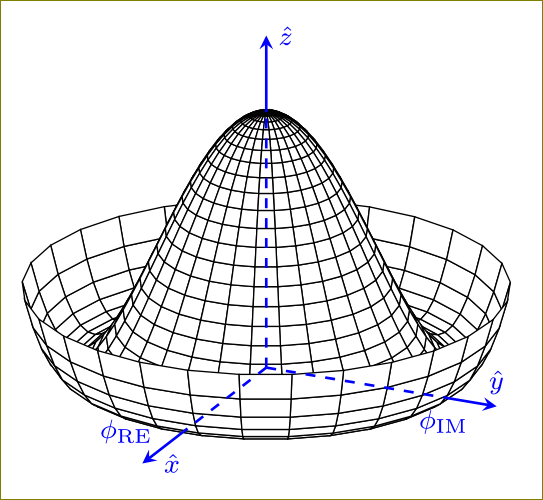
\includegraphics[width=0.4\linewidth]{figures/theory/higgs_potential.png}
    \caption{ A lower-dimensionality representation of the shape of the Higgs
potential.  The central peak represents a rotationally symmetric
unstable state, while the trough represents the infinite number of minima that
can be selected upon the spontaneous breaking of the symmetry.}
    \label{fig:higgs_potential}
  \end{center}
\end{figure}

The value of this minima can be calculated by taking the derivative of V with
respect to $\boldsymbol{\Phi}$ and setting it equal to $0$. This value, also
known as the vacuum expectation value (vev) has been found to be $v \equiv
\sqrt{-\mu^{2}/\lambda} = 246$ GeV. The arbitrary vev of the ground state Higgs
field is acquired when the symmetry of the Higgs potential is spontaneously broken.
For ease of calculation the coordinate system is oriented such that

\begin{equation}
\left\langle \boldsymbol{\Phi}(x) \right\rangle = \frac{1}{\sqrt{2}} \left(
\begin{matrix} 0 \\ v \end{matrix} \right)
\end{equation} 

Next small perturbations around the minimum of the Higgs
potential are parameterized as 

\begin{equation} \label{eq:higgs:broken_higgs}
\left\langle \boldsymbol{\Phi}(x) \right\rangle = \frac{1}{\sqrt{2}} \left(
\begin{matrix} 0 \\ v + h(x) \end{matrix} \right) \text{exp} \left(
i\frac{\tau^{i}}{2}\theta^{i}(x) \right)
\end{equation} 

Here the real scalar field $h(x)$ corresponds to radial perturbations of the
minima, and the three $\theta^{i}(x)$ are the Nambu-Goldstone fields with
values determined by the choice of gauge.  Choosing the unitary gauge of
$\theta^{i}(x) = 0$ and expanding the kinetic term of
\Cref{eq:higgs:lagrangian} around the vev gives

\begin{equation} \label{eq:higgs:boson_masses}
\mathcal{L}_{\text{Higgs},K} = \frac{g^{2}v^{2}}{8} \left(
(W_{\mu}^{-})^{\dagger}W^{-\mu} + (W_{\mu}^{+})^{\dagger}W^{+\mu} \right) +
\frac{1}{2} \left( \begin{matrix} W_{\mu}^{3\dagger} & B_{\mu}^{\dagger}
\end{matrix} \right) \boldsymbol{M}^{2} \left( \begin{matrix} W^{3\mu} \\ B^{\mu}
\end{matrix} \right) + \ldots 
\end{equation}

Here the first term is the physical mass term for the $W^{\pm}$ bosons where
these charge eigenstates have been constructed out of the $W^{1,2}$ fields as
such $W^{\pm} = \frac{1}{\sqrt{2}}(W^{1} \mp iW^{2})$.  The second term
represents the mixture of the $W^{3}$ and $B$ fields through the mass matrix
$\boldsymbol{M}$.  Diagonalizing this matrix ($M_{D}$) and identifying the mass
eigenstates gives the physical fields of the photon ($\gamma$) and the $Z$
boson


\begin{equation}
\boldsymbol{M}_{D}^{2} = \left( \begin{matrix} 0 & 0 \\ 0 &
\frac{v^{2}}{4}(g_{W}^{2} + g^{'2)}   \end{matrix} \right)
\end{equation}

The upper left diagonal element corresponds to the massless photon
while the lower right diagonal element gives the mass of the massive $Z$ boson.
This leaves us with the following masses for the 4 electroweak bosons

\begin{equation}
m_{W} = \frac{1}{2}g_{W}v \quad , \quad m_Z = \frac{1}{2}v\sqrt{g_{W}^{2} + g^{'2}}
\quad , \quad m_\gamma = 0
\end{equation}

The masses of the $W^{\pm}$ and $Z$ gauge bosons can be related through the
Weinberg mixing angle defined as

\begin{equation}
\theta_W = \cos^{-1}\left( \frac{g_{W}}{\sqrt{g_{W}^{2}+g^{'2}}} \right) \rightarrow m_{Z} =
\frac{m_{W}}{\cos{\theta_{W}}}
\end{equation}

Using this definition one can write out the exact mixture of $B$ and $W^{3}$ that
make up the photon and $Z$ boson as

\begin{align}
\gamma &= \text{cos}(\theta_{W})B + \text{sin}(\theta_{W})W^{3} \\
Z &= -\text{sin}(\theta_{W})B + \text{cos}(\theta_{W})W^{3}
\end{align}

\subsection{Fermion Mass Terms} \label{sec:theory:fermion_mass}

\Cref{sec:theory:gsw} shows how a simple fermion mass terms violate gauge
invariance due to the mixing of the left and right chiral states.  The Higgs
mechanism, however, allows for a gauge-invariant method of generating mass
terms through the Yukawa coupling of the Higgs field to the fermion fields.  An
example is the Yukawa coupling term for the electron doublet
($\boldsymbol{\Psi}_{L}$) and singlet ($\Psi_R$) coupling to the Higgs field
($\boldsymbol{\Phi}$) after spontaneous symmetry breaking, with the form
shown in \Cref{eq:higgs:broken_higgs}, when the unitary gauge $\Phi^{i}(x) = 0$
is chosen.

\begin{align}
\mathcal{L}_{\text{Yukawa}} &= - g_{e} \left[ \boldsymbol{\bar{\Psi}_L}
\boldsymbol{\Phi} \Psi_R + \bar{\Psi}_{R} \boldsymbol{\Phi}^{\dagger} \boldsymbol{\Psi_L}
\right] \\ &= - \frac{g_{e}}{\sqrt{2}} \left[ \left( \begin{matrix}
\bar{\nu}_{e} & \bar{e} \end{matrix} \right)_L \left( \begin{matrix} 0 \\ \nu +
h \end{matrix} \right) e_{R} + \bar{e}_{R} \left( \begin{matrix} 0 & (\nu + h)
\end{matrix} \right) \left( \begin{matrix} \nu_{e} \\ e \end{matrix} \right)_L \ \right] \\ &= - \underbrace{\frac{g_{e}}{\sqrt{2}}
\nu}_{m_{e}} \left( \bar{e}_{L}e_{R} + \bar{e}_{R}e_{L}  \right)
- \underbrace{\frac{g_{e}}{\sqrt{2}}}_{g_{e,h}} h \left(
\bar{e}_{L}e_{R} + \bar{e}_{R}e_{L}  \right) 
\end{align}

In this way mass terms are generated for the fermion field and the gauge
invariance of the Lagrangian is maintained by using only gauge invariant
fields.  This operation has also left us with the second term which represents
the coupling of the electron to the higgs itself thus giving us the form of its
coupling constant $g_{e,h}$.  Using this newly found mass of the electron
$m_{e}$ the coupling can be written as

\begin{equation}
g_{e,h} = \frac{g_{e}}{\sqrt{2}} = \frac{m_{e}}{\nu}.
\end{equation}

Thus the coupling of the Higgs boson to a fermion is proportional
to the mass of the fermion itself. 
 
\subsection{The Higgs Boson}

The Higgs mechanism not only properly mixes the gauge fields to provide the
correct gauge-invariant mass terms, but also properly combines the left and
right chiral states of fermions to produce their mass terms. Furthermore, the 4
degrees of freedom in the Higgs doublet (\Cref{eq:higgs:higgs_field} become
physical particles, known as the Goldstone bosons, during the spontaneous
breaking of the electroweak potential \cite{Higgs:1964pj}.  Three of these
Goldstone bosons are ``eaten" by the 3 gauge bosons $W^{\pm}$ and $Z$ to form
their longitudinal components thus give them their mass. The final broken
degree of freedom is absorbed by the new massive scalar particle, the Higgs
boson \cite{Higgs:1964pj}.

Focusing on the potential term (V) of
\Cref{eq:higgs:lagrangian} and substituting in the definition for
$\boldsymbol{\Phi}$ given in \Cref{eq:higgs:broken_higgs} gives

\begin{equation}
\mathcal{L}_\text{Higgs,V} = \frac{1}{2} \mu^{2} \nu^{2} - \mu^{2} h^{2} +
\lambda \nu h^{3} + \frac{1}{4} \lambda h^{4}
\end{equation}

The first term is constant and thus can be ignored.  The second term is the
mass term for the Higgs boson, $m_h = \sqrt{-2\mu^{2}} = \sqrt{2\lambda}\nu$.
Remembering that $h = h(x)$ was used for small radial perturbations of the
Higgs field the Higgs boson can be identified as a radial excitation of the
Higgs field.  Finally, the third and fourth terms represent the Higgs boson
self-couplings.  With these couplings and mass terms in hand the next step is
to experimentally verify this theory as discussed next in \Cref{chap:higgs}.
